\begin{center}
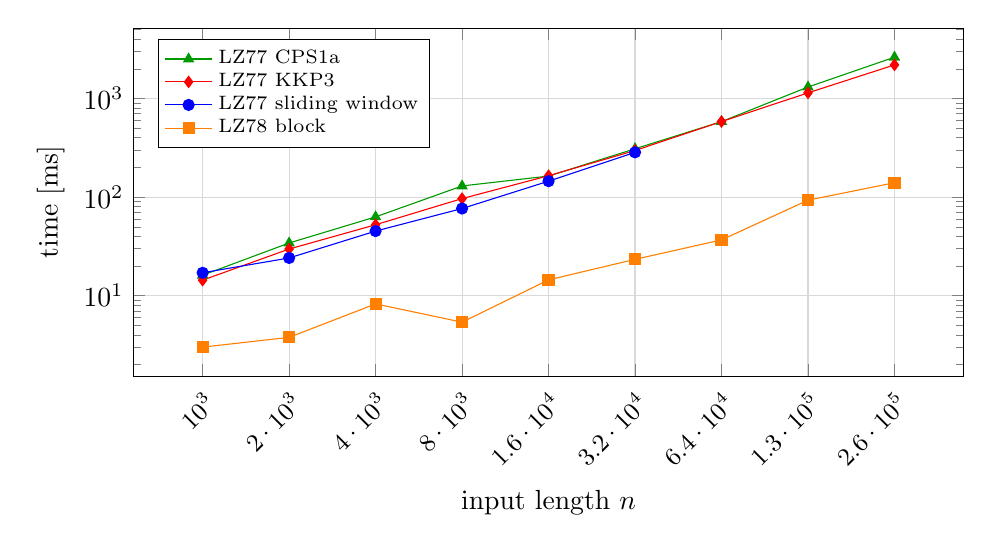
\begin{tikzpicture}
\begin{axis}[
  width = \linewidth, height = 6cm,
  xlabel = {input length $n$}, ylabel = {time [ms]},
  xmode = log, ymode = log,
  legend pos = north west, legend cell align = left,
  legend style = {font = \scriptsize, row sep = -2pt, inner sep = 2pt},
  xmajorgrids = true, ymajorgrids = true,
  xminorgrids = false, yminorgrids = false,
  minor tick num = 0,
  grid style = {draw = gray!30},
  xtick = {1000, 2000, 4000, 8000, 16000, 32000, 64000, 128000, 256000},
  xticklabels = {$10^{3}$, $2 \cdot 10^{3}$, $4 \cdot 10^{3}$, $8 \cdot 10^{3}$, $1.6 \cdot 10^{4}$, $3.2 \cdot 10^{4}$, $6.4 \cdot 10^{4}$, $1.3 \cdot 10^{5}$, $2.6 \cdot 10^{5}$},
  x tick label style = {rotate = 45, anchor = north east, font = \small},
]
\addplot[color = green!60!black, mark = triangle*] coordinates {(1000, 16.14) (2000, 34.24) (4000, 63.02) (8000, 129.76) (16000, 163.47) (32000, 309.23) (64000, 582.9) (128000, 1307.41) (256000, 2622.61)};
\addlegendentry{LZ77 CPS1a}
\addplot[color = red, mark = diamond*] coordinates {(1000, 14.38) (2000, 29.74) (4000, 52.43) (8000, 96.62) (16000, 164.66) (32000, 296.95) (64000, 583.29) (128000, 1140.96) (256000, 2190.97)};
\addlegendentry{LZ77 KKP3}
\addplot[color = blue, mark = *] coordinates {(1000, 17.09) (2000, 24.14) (4000, 45.24) (8000, 76.6) (16000, 145.07) (32000, 284.37)};
\addlegendentry{LZ77 sliding window}
\addplot[color = orange, mark = square*] coordinates {(1000, 3.01) (2000, 3.78) (4000, 8.26) (8000, 5.39) (16000, 14.47) (32000, 23.38) (64000, 36.82) (128000, 93.05) (256000, 139.94)};
\addlegendentry{LZ78 block}
\end{axis}
\end{tikzpicture}
\captionof{figure}{Thue-Morse, encoding time.}
\label{fig:Thue-Morse-encoding}
\end{center}

\begin{center}
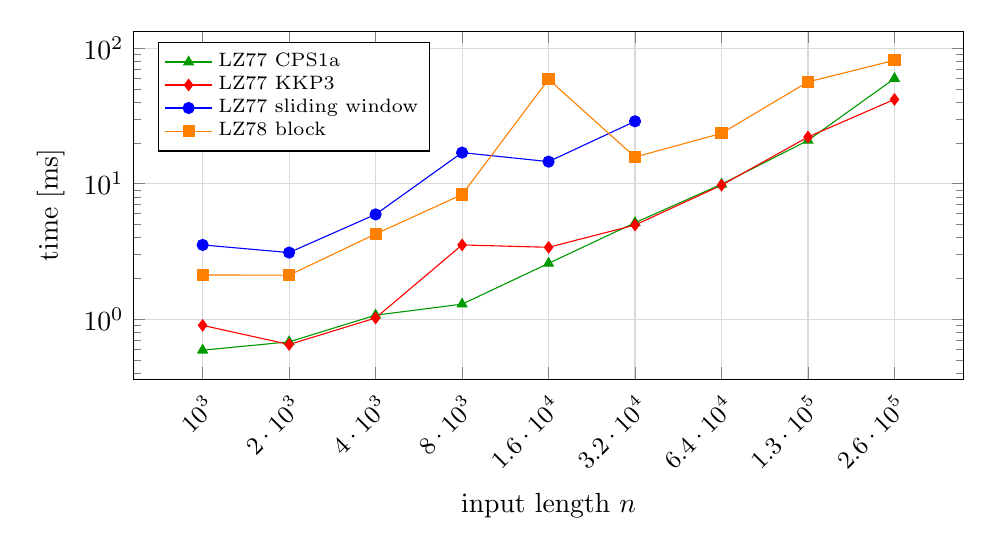
\begin{tikzpicture}
\begin{axis}[
  width = \linewidth, height = 6cm,
  xlabel = {input length $n$}, ylabel = {time [ms]},
  xmode = log, ymode = log,
  legend pos = north west, legend cell align = left,
  legend style = {font = \scriptsize, row sep = -2pt, inner sep = 2pt},
  xmajorgrids = true, ymajorgrids = true,
  xminorgrids = false, yminorgrids = false,
  minor tick num = 0,
  grid style = {draw = gray!30},
  xtick = {1000, 2000, 4000, 8000, 16000, 32000, 64000, 128000, 256000},
  xticklabels = {$10^{3}$, $2 \cdot 10^{3}$, $4 \cdot 10^{3}$, $8 \cdot 10^{3}$, $1.6 \cdot 10^{4}$, $3.2 \cdot 10^{4}$, $6.4 \cdot 10^{4}$, $1.3 \cdot 10^{5}$, $2.6 \cdot 10^{5}$},
  x tick label style = {rotate = 45, anchor = north east, font = \small},
]
\addplot[color = green!60!black, mark = triangle*] coordinates {(1000, 0.59) (2000, 0.68) (4000, 1.07) (8000, 1.29) (16000, 2.58) (32000, 5.15) (64000, 9.9) (128000, 20.85) (256000, 59.68)};
\addlegendentry{LZ77 CPS1a}
\addplot[color = red, mark = diamond*] coordinates {(1000, 0.9) (2000, 0.65) (4000, 1.02) (8000, 3.53) (16000, 3.39) (32000, 4.95) (64000, 9.74) (128000, 22.11) (256000, 41.88)};
\addlegendentry{LZ77 KKP3}
\addplot[color = blue, mark = *] coordinates {(1000, 3.53) (2000, 3.1) (4000, 5.93) (8000, 16.95) (16000, 14.54) (32000, 28.85)};
\addlegendentry{LZ77 sliding window}
\addplot[color = orange, mark = square*] coordinates {(1000, 2.12) (2000, 2.11) (4000, 4.25) (8000, 8.31) (16000, 58.87) (32000, 15.72) (64000, 23.51) (128000, 56.39) (256000, 81.38)};
\addlegendentry{LZ78 block}
\end{axis}
\end{tikzpicture}
\captionof{figure}{Thue-Morse, decoding time.}
\label{fig:Thue-Morse-decoding}
\end{center}

\begin{center}
\begin{tabular}{lrrrrrr}
\hline
algorithm & $n$ & $\alpha$ & $z$ & $\rho$ & encode [ms] & decode [ms] \\
\hline
LZ77 sliding window & 32000 & 2 & 29 & 0.0281 & 461.67 & 49.65 \\
LZ78 block & 32000 & 2 & 1425 & 0.4704 & 29.4 & 26.28 \\
LZ77 CPS1a & 32000 & 2 & 29 & 0.0263 & 448.91 & 8.45 \\
LZ77 KKP3 & 32000 & 2 & 29 & 0.0263 & 410.0 & 8.69 \\
\hline
\end{tabular}
\captionof{table}{Thue-Morse: the Thue-Morse word.}
\label{tab:Thue-Morse}
\end{center}